Aquí vamos a hacer una comparativa preliminar del conjunto de funciones presentado junto con sus versiones de dos y cuatro fuentes. 

\begin{itemize}
    \item \textbf{A. Comparación por número de fuentes}

La documentación utilizada y los recursos citados en este prroyecto en múltipples ocasiones comentan las diferencias entre estos dos enfoques al problema.
La separación que resulta en el conjunto de dos fuentes, ya visto en las primeras versiones del entrenamiento, es un enfoque más sencillo que permite una "binarización" del problema al reducirse a dos salidas. En contraposición con el segundo conjunto, donde la separación se exxxtiende a identificar cuatro elementos en el espectro, los elementos que se puedan identificar si el método es válido pueden variar enormemente dificultando así la identificación de estos, ya que, un elemento que a lo mejor está en un rango
frecuencial concreto en una mezcla, en otra puede habitar en otro no a lo mejor completamente diferente pero sí lo suficiente para que la sensibilidad de la función a estos cambios no dé al modelo la información necesaria para ser capaz de identificar un elemento que varía.
Por esto, es esperable que, por lo general, \textit{4 stems} obtenga peores métricas en la fase de evaluación. Identificar y separar dos elementos en contraposición y por lo comentado, resulta en una tarea más sencilla ya que la variabilidad se reduce a eso, dos elementos, mientras que el caso anterior eleva la premisa de la necesidad de sensibilidad en la función al doble de elementos donde puede variar este rango frecuencial.

Por ejemplo , géneros como la electrónica o el rap que se basan en elementos frecuencialmente bajos ( bajo, sub-bajo ) presentan gran superposición entre fuentes como bajo y baterías, es un sonido más "sucio" y armónicamente complejo.
Por otro lado, por ejemlo, el blues, pop, o canciones de autor, presentan mejores desempeños en la separación por sus características de armónicos vocales e instrumentales más limpios \cite{Arxiv}.

\begin{figure}[H]
    \begin{center}
    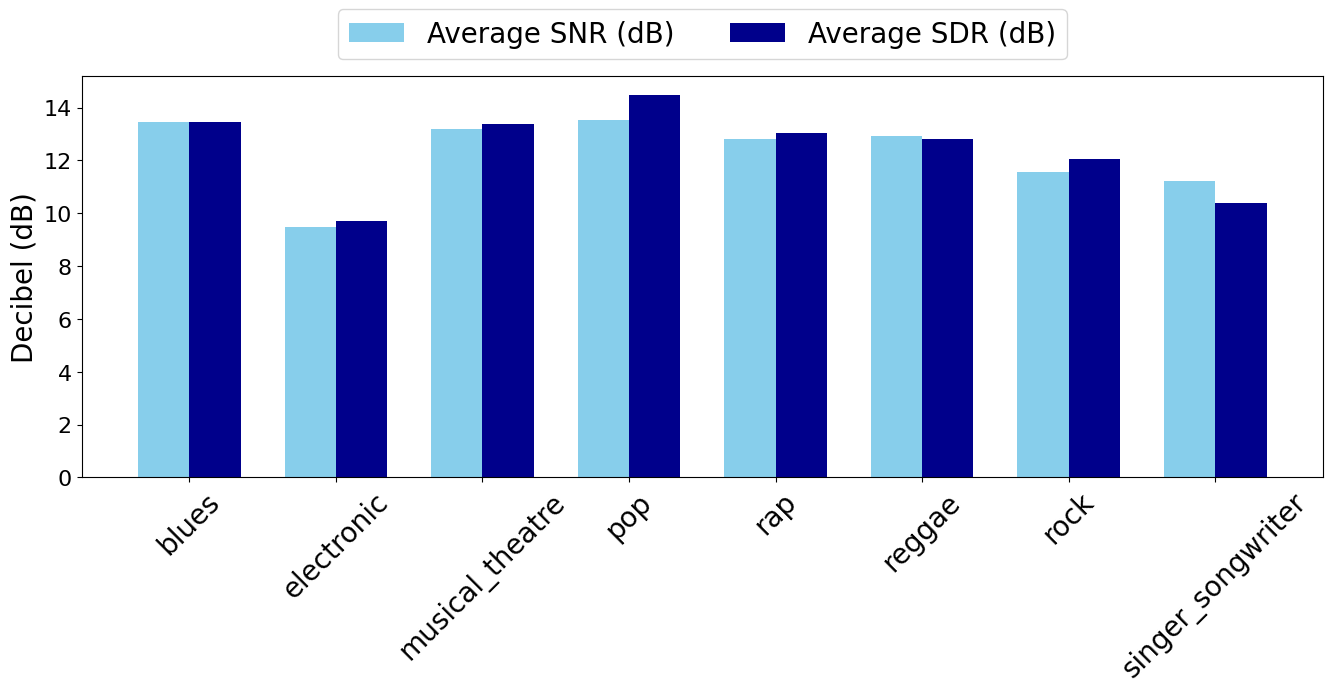
\includegraphics[width=0.7\textwidth]{commons/Fig10.png}
    \caption{Average SNR and SDR by genre}
    \label{fig:SNR SDR by genre}
    \end{center}
\end{figure}

    \item \textbf{B. Comparación por familia de pérdida}

Se han agrupado las funciones de pérdida por las familias aritméticas a las que pertenecen por su naturaleza:

    \begin{itemize}
        \item Pérdidas de magnitud directa: L1 , L2.
        \item Pérdidas frecuenciales: L1\_freq, L2\_freq.
        \item Pérdidas logarítmicas: logL1, logL2, log\_mag, log\_compressed\_l2.
        \item Pérdidas informadas por fase o potencia: LPSA, lpsa\_phase.
        \item Pérdidas basadas en máscara: mask\_l1
        \item Pérdidas experimentales: deep\_feature , deep\_feature\_emd
    \end{itemize}

Las pérdidas logarítmicas buscan reducir el efecto de diferencias absolutas grandes en \textit{bins} energéticos y prestar más atención a estructuras de menor energía.
Las frecuenciales, comparan directamente la representación tiempo-frecuencia, mientras que las basadas en máscara fuerzan al modelo a aproximar una asignación explícita de cada bin a una fuente.


\end{itemize}